\section{\texttt{simpleStatisticalForwardProblem}}\label{sec:example_sfp}

In this simple statistical forward problem (SFP), suppose that the quantity of interest $\mathbf{q}$ is a function of a random variable $\bv{\theta}$ of two parameters, namely $\bf{q}:\mathbb{R}^2\rightarrow\mathbb{R}$ such as:
\begin{equation}\label{eq-example-q}
\mathbf{q}(\boldsymbol{\theta}) = \theta_1+\theta_2,\quad\forall\boldsymbol{\theta}=(\theta_1,\theta_2)\in\mathbb{R}^2.
\end{equation}

Suppose also that the parameters in $\theta$ have Gaussian distribution with mean $\bv{\mu}$ and covariance matrix $\bf{C}$ given by:
\begin{equation}\label{eq-example-mu-sfp}
\boldsymbol{\mu} = 
\left(\begin{array}{c}
-1 \\
2
\end{array}\right)
\quad
\text{and}
\quad
\mathbf{C} = 
\left[\begin{array}{cc}
4 & 0 \\
0 & 1
\end{array}\right].
\end{equation}


Notice that since the solution $\mathbf{Q}$ of this SFP is the sum of two random variables $\boldsymbol{\Theta}_1$ and $\boldsymbol{\Theta}_2$, and since these two random variables independent Gaussian by assumption, should have:
\begin{equation}\label{eq-example-E-V}
E[\mathbf{Q}] = E[\boldsymbol{\Theta}_1] + E[\boldsymbol{\Theta}_2] = -1 + 2 = 1 \quad \text{and} \quad
%
V[\mathbf{Q}] = V[\boldsymbol{\Theta}_1] + V[\boldsymbol{\Theta}_2] = 4 + 1 = 5
\end{equation}
% and
% \begin{equation}\label{eq-example-V}
% V[\mathbf{Q}] = V[\boldsymbol{\Theta}_1] + V[\boldsymbol{\Theta}_2] = 4 + 1 = 5
% \end{equation}
where $E$ and $V$ indicate expectation and variance, respectively. Thus the analytical expression for the solution $\bf{Q}$ is this SFP is the one-dimensional Gaussian distribution of mean 1 and variance 5:
\begin{equation}\label{eq-example-sfp-analytical}
{\bf Q}(x)=   \frac{1}{ \sqrt{10\pi}} \exp\left(-\frac{1}{10}(x-1)^2 \right)
\end{equation}


In this example, we use QUESO Monte Carlo algorithm to sample from the QoI given in Equation (\ref{eq-example-q}) and analyze it. 
Since the parameters have known independent Gaussian distributions, the results obtained by QUESO via sampling the QoI, in Equation (\ref{eq-example-q}), should match the Gaussian distribution given in Equation (\ref{eq-example-sfp-analytical}).


\paragraph*{Note:} Due to the possibility to compare QUESO sampling algorithms to an analytical expression, this example is also used in the verification procedures and regression tests within QUESO. In fact it is the second part of the test \verb+tests/t02_sip_sfp+.


\subsection{Running the Example}\label{sec:sfp-run}
 
To run the executable provided (available after QUESO installation), enter the following commands:
\begin{lstlisting}[label={},caption={}]
$ cd $HOME/LIBRARIES/QUESO-0.51.0/
$ cd examples/simpleStatisticalForwardProblem
$ rm outputData/*
$ ./exSimpleStatisticalForwardProblem_gsl example.inp    
$ matlab
   $ simple_fp_plots      # inside matlab
   $ exit                 # inside matlab
$ ls -l outputData/*.png
 simple_fp_autocorrelation_qoi.png  simple_fp_chain_pos_param.png  
 simple_fp_hist_qoi.png             simple_fp_cdf_qoi.png
 simple_fp_chain_pos_qoi.png        simple_fp_kde_qoi.png
\end{lstlisting}

As a result, the user should have created several of PNG figures containing marginal posterior PDF, chain positions of the parameters and the QoI, histogram, cumulative density distribution and autocorrelation. The name of the figure files have been chosen to be informative, as shown in the Listing above.



\subsection{Example Code}\label{sec:code-sfp}

The source code for the SFP example is composed of 5 files:
\texttt{simple\_sfp\_example\_main.C} (Listing~\ref{code:sfp-main-c}),
\texttt{simple\_sfp\_example\_qoi.h} and \texttt{simple\_sfp\_example\_qoi.C} (Listings \ref{code:sfp-qoi-h} and~\ref{code:sfp-qoi-c}),
\texttt{simple\_sfp\_example\_compute.h}  and \texttt{simple\_sfp\_example\_compute.C} (Listings \ref{code:sfp-compute-h} and \ref{code:sfp-compute-c}).


\lstinputlisting[caption=File \texttt{simple\_sfp\_example\_main.C.}, label={code:sfp-main-c}, linerange={25-1000}]{../../examples/simpleStatisticalForwardProblem/src/simple_sfp_example_main.C}

\lstinputlisting[caption=File \texttt{simple\_sfp\_example\_qoi.h}., label={code:sfp-qoi-h}, linerange={25-1000}]{../../examples/simpleStatisticalForwardProblem/src/simple_sfp_example_qoi.h}

\lstinputlisting[caption=File \texttt{simple\_sfp\_example\_qoi.C}., label={code:sfp-qoi-c}, linerange={25-1000}]{../../examples/simpleStatisticalForwardProblem/src/simple_sfp_example_qoi.C}

\lstinputlisting[caption=File \texttt{simple\_sfp\_example\_compute.h.}, label={code:sfp-compute-h}, linerange={25-1000}]{../../examples/simpleStatisticalForwardProblem/src/simple_sfp_example_compute.h}

\lstinputlisting[caption={File \texttt{simple\_sfp\_example\_compute.C}.}, label={code:sfp-compute-c}, linerange={25-1000},numbers=left]{../../examples/simpleStatisticalForwardProblem/src/simple_sfp_example_compute.C}
 


\subsection{Input File}\label{sec:sfp-input-file}

In the case of a SFP, QUESO expects a list of options for Monte Carlo algorithm,
together with options for QUESO environment; such as the name of the output files and which sub-environments will write to to them. 
Note that the names of the variables have been designed to be informative:
\begin{description}\vspace{-8pt}
\item[ \texttt{env}:] refers to QUESO environment; \vspace{-8pt}
\item[ \texttt{fp}:] refers to forward problem;\vspace{-8pt}
\item[ \texttt{mc}:] refers to Monte Carlo;\vspace{-8pt}
\item[ \texttt{pseq}:] refers to the parameter sequence; and\vspace{-8pt}
\item[ \texttt{qseq}:] refers to the quantity of interest sequence.
\end{description}

The options used for solving this simple SFP are displayed in Listing \ref{code:sfp-input-file}.


\lstinputlisting[caption={File name \texttt{simple\_sfp\_example.inp} with options for QUESO library used in application code (Listings \ref{code:sfp-main-c}--\ref{code:sfp-compute-c}})., 
label={code:sfp-input-file},]{../../examples/simpleStatisticalForwardProblem/tests/test_2013_08_27/simple_sfp_example.inp}



\subsection{Create your own Makefile}\label{sec:sfp-makefile}

 
Listing \ref{code:makefile} presents a Makefile, named `\texttt{Makefile\_sfp\_example\_margarida}', that may be used to compile the code and create the executable \verb+simple_sfp_example+. Naturally, it must be adapted to the user's settings, i.e., it has to have the correct paths for the user's libraries that have actually been used to compile and install QUESO.

\begin{lstlisting}[caption={Makefile for the application code in Listings
  \ref{code:sfp-main-c}--\ref{code:sfp-compute-c}},
  label={code:sfp-makefile},
  language={bash}]
  QUESO_DIR = /path/to/queso
  BOOST_DIR = /path/to/boost
  GSL_DIR   = /path/to/gsl

  INC_PATHS = \
     -I. \
     -I$(QUESO_DIR)/include \
     -I$(BOOST_DIR)/include \
     -I$(GSL_DIR)/include

  LIBS = \
     -L$(QUESO_DIR)/lib -lqueso \
     -L$(BOOST_DIR)/lib -lboost_program_options \
     -L$(GSL_DIR)/lib -lgsl

  CXX = mpic++
  CXXFLAGS += -g -Wall -c

  default: all

  .SUFFIXES: .o .C

  all:       example_sfp

  clean:
     rm -f *~
     rm -f *.o
     rm -f simple_sfp_example

  example_sfp: simple_sfp_example_main.o simple_sfp_example_qoi.o simple_sfp_example_compute.o
     $(CXX) simple_sfp_example_main.o \
            simple_sfp_example_qoi.o \
            simple_sfp_example_compute.o \
            -o simple_sfp_example $(LIBS)

  %.o: %.C
     $(CXX) $(INC_PATHS) $(CXXFLAGS) $<
\end{lstlisting}

Thus, to compile, build and execute the code, the user just needs to run the following commands in the same directory where the files are:
\begin{lstlisting}
$ cd HOME/LIBRARIES/QUESO-0.51.0/examples/simpleStatisticalForwardProblem 
$ export LD_LIBRARY_PATH=$LD_LIBRARY_PATH:\
  $HOME/LIBRARIES/gsl-1.15/lib/:\
  $HOME/LIBRARIES/boost-1.53.0/lib/:\
  $HOME/LIBRARIES/hdf5-1.8.10/lib:\
  $HOME/LIBRARIES/QUESO-0.51.0/lib 
$ make -f Makefile_sfp_example_margarida 
$ ./simple_sfp_example simple_sfp_example.inp
\end{lstlisting}

The `\verb+export+' instruction above is only necessary if the user has not saved it in his/her \verb+.bashrc+ file. 


\subsection{Data Post-Processing and Visualization}\label{sec:sfp-results}

This section discusses the results computed by QUESO with the code of Section \ref{sec:code-sfp}, and shows how to use Matlab for the post-processing of the data generated by QUESO when solving SFPs. Only the essential Matlab commands are presented; for the complete/detailed codes, please refer to file '\verb+simple_fp_plots.m+'.

According to the specifications of the input file in Listing~\ref{code:sfp-input-file}, a folder named `\verb+outputData+' containing the following files should be created: \verb+display_sub0.txt, fp_p_seq.m,+ \linebreak \verb+fp_p_seq_sub0.m, fp_q_seq.m, fp_q_seq_sub0.m,+ and \verb+sfpOutput_sub0.m+.

The code below shows how to load the data provided by QUESO during the solution
process of the SFP described, in the form of chains of positions.
\begin{lstlisting}[caption={Matlab code for loading the data in both parameter and QoI chains of the SFP.}]
% inside Matlab
>> clear all
>> fp_p_seq.m
>> fp_q_seq.m
\end{lstlisting}


Alternatively, the user may call the file \texttt{simple\_fp\_plots.m}, which
contains the above commands, together with a variety of others, for data
visualization:
\begin{lstlisting}[caption={Matlab code for loading the data in both parameter and QoI chains of the SFP, by calling the file \texttt{simple\_fp\_plots.m}.}]
% inside Matlab
>> clear all
>> simple_fp_plots
\end{lstlisting}




\subsubsection{Histogram Plots}

In order to plot a histogram of the QoI, you may use the pre-defined Matlab function \verb+hist+.
The Matlab code presented in Listing \ref{matlab:fp_hist_qoi} below shows how to create the Figure~\ref{fig:fp_qoi_hist}.

\begin{lstlisting}[label=matlab:fp_hist_qoi,caption={Matlab code for the QoI histogram plot.}]
% inside Matlab
>> fp_q_seq  %if commands of Listings 3.19/3.20 have not been called
>> nbins=20;
>> hist(fp_mc_QoiSeq_unified,nbins);
>> title('QoI Histogram','fontsize',20);
>> xlabel('QoI=\theta_1+\theta_2','fontname', 'Times', 'fontsize',20)
>> ylabel('Frequency','fontsize',20);
\end{lstlisting}

\begin{figure}[p]
\centering 
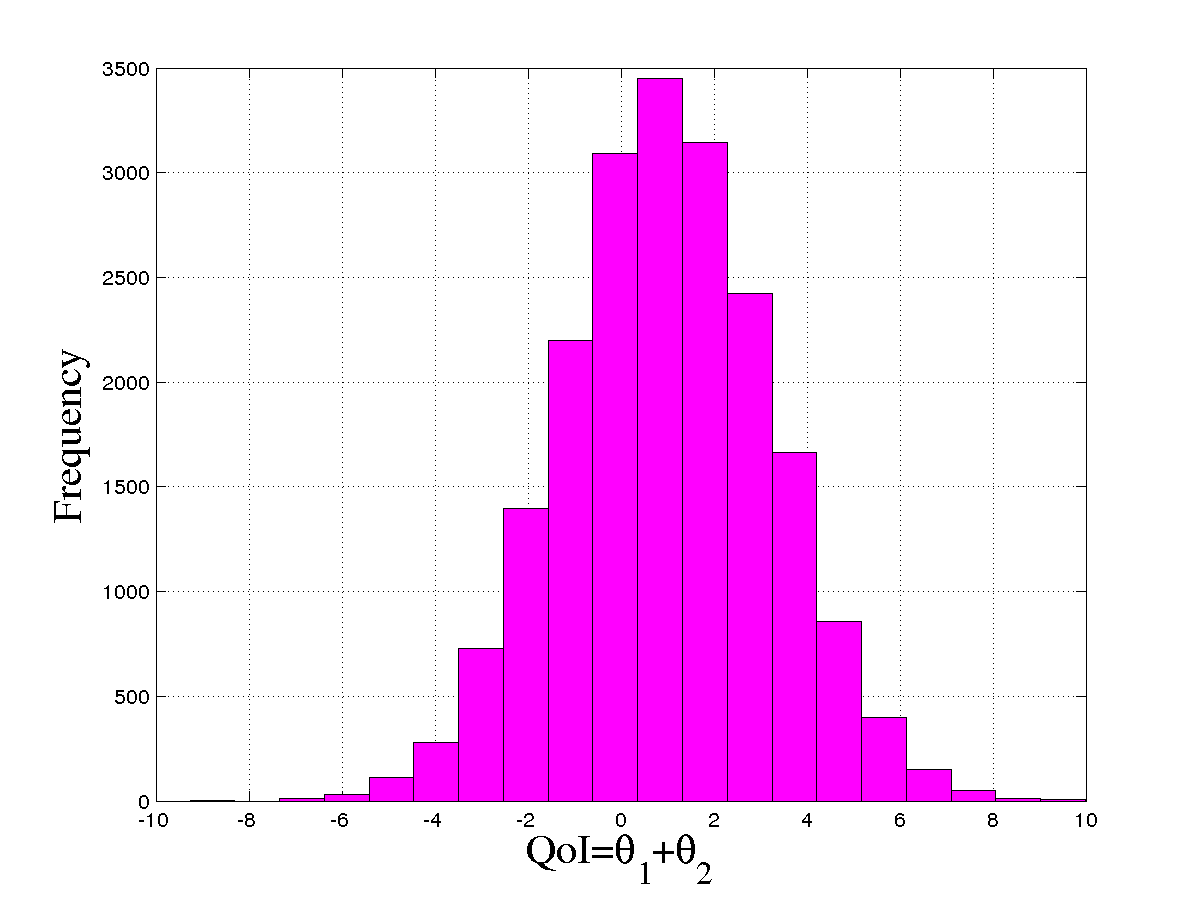
\includegraphics[scale=0.35]{figs/simple_fp_hist_qoi.png}
\vspace{-10pt}
\caption{QoI histogram.}
\label{fig:fp_qoi_hist}
\end{figure}

\subsubsection{KDE Plot}

Matlab function \verb+ksdensity+ (Kernel smoothing density estimate) together with the option `\verb+pdf+' may be used to estimate the KDE of the QoI. 

\begin{lstlisting}[label=matlab:fp_kde_qoi,caption={Matlab code for the KDE displayed in Figure \ref{fig:simple_sfp_kde}}]
% inside Matlab
>> fp_q_seq  %if commands of Listing 5.19 have not been called
>> [fi,xi] = ksdensity(fp_mc_QoiSeq_unified,'function','pdf');
>> x=sort(fp_mc_QoiSeq_unified);
>> mu=1;
>> sigma2=5;
>> f=(exp(-(x-mu).*(x-mu)/sigma2/2))/sqrt(2*pi*sigma2);
>> plot(xi,fi,'-m','linewidth',4);
>> hold;
>> plot(x,f,'--k','linewidth',2);
>> h=legend('QoI = \theta_1+\theta_2','analytical','location','northwest');
\end{lstlisting}


%Figure \ref{fig:sip_gravity_kde_raw} is created by using Matlab commands presented in Listing \ref{matlab:kde} above.
\begin{figure}[p]
\centering 
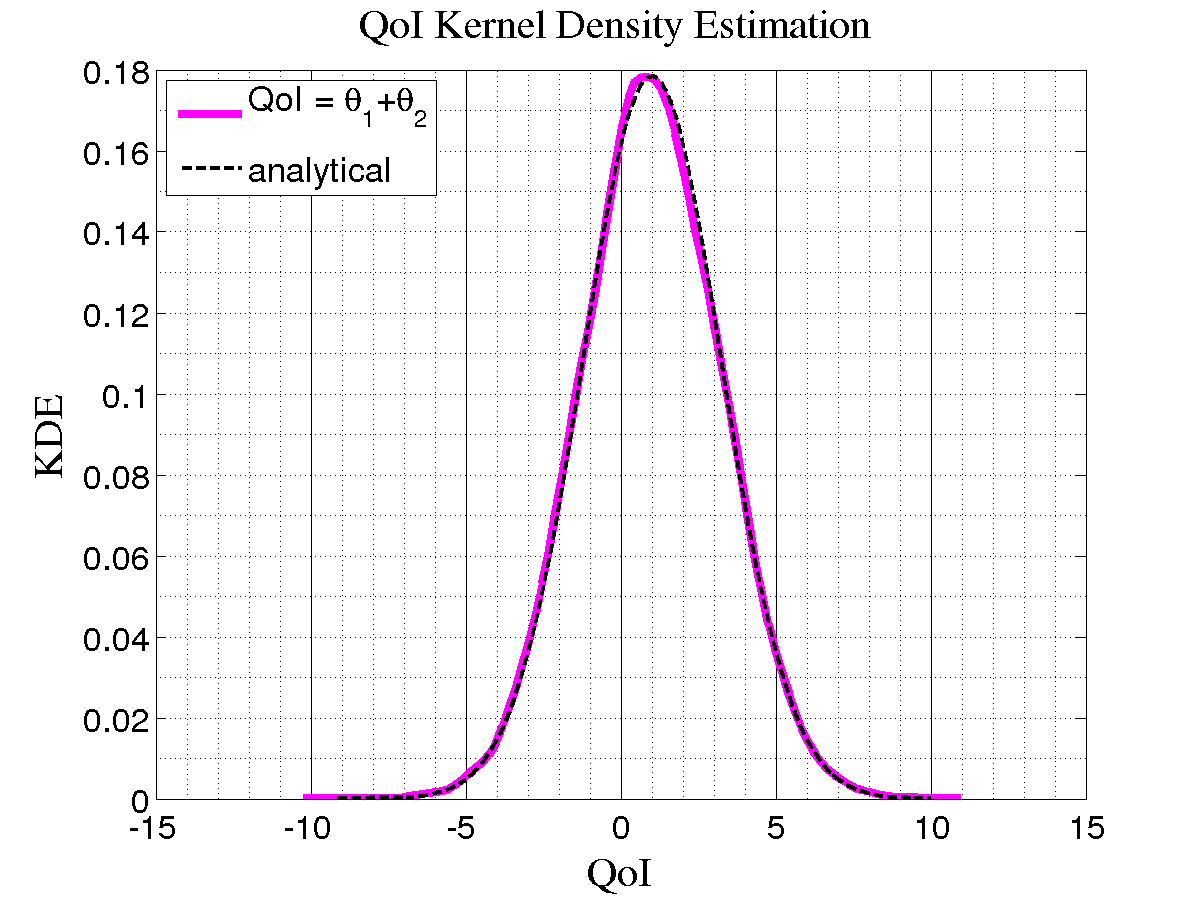
\includegraphics[scale=0.35]{figs/simple_fp_kde_qoi.png}
\vspace{-10pt}
\caption{Kernel Density Estimation. QUESO results are plotted against the PDF of a Gaussian distribution $Q(x)=   \frac{1}{ \sqrt{10\pi}} \exp\left(-\frac{1}{10}(x-1)^2 \right)$, where $\mu=1$ and $\sigma^2=5$.}
\label{fig:simple_sfp_kde}
\end{figure}


\subsubsection{CDF Plot}

Matlab function \verb+ksdensity+ with \verb+'cdf'+ option may also be used for plotting the Cumulative Distribution Function of the QoI.

\begin{lstlisting}[label=matlab:fp_cdf_qoi,caption={Matlab code for the QoI CDF plot displayed in Figure \ref{fig:simple_sfp_cdf}.}]
% inside Matlab
>> fp_q_seq  %if commands of Listing 5.19 have not been called
>> [f,xi] = ksdensity(fp_mc_QoiSeq_unified,'function','cdf');
>> plot(xi,f,'-m','linewidth',3)
\end{lstlisting}

\begin{figure}[p]
\centering 
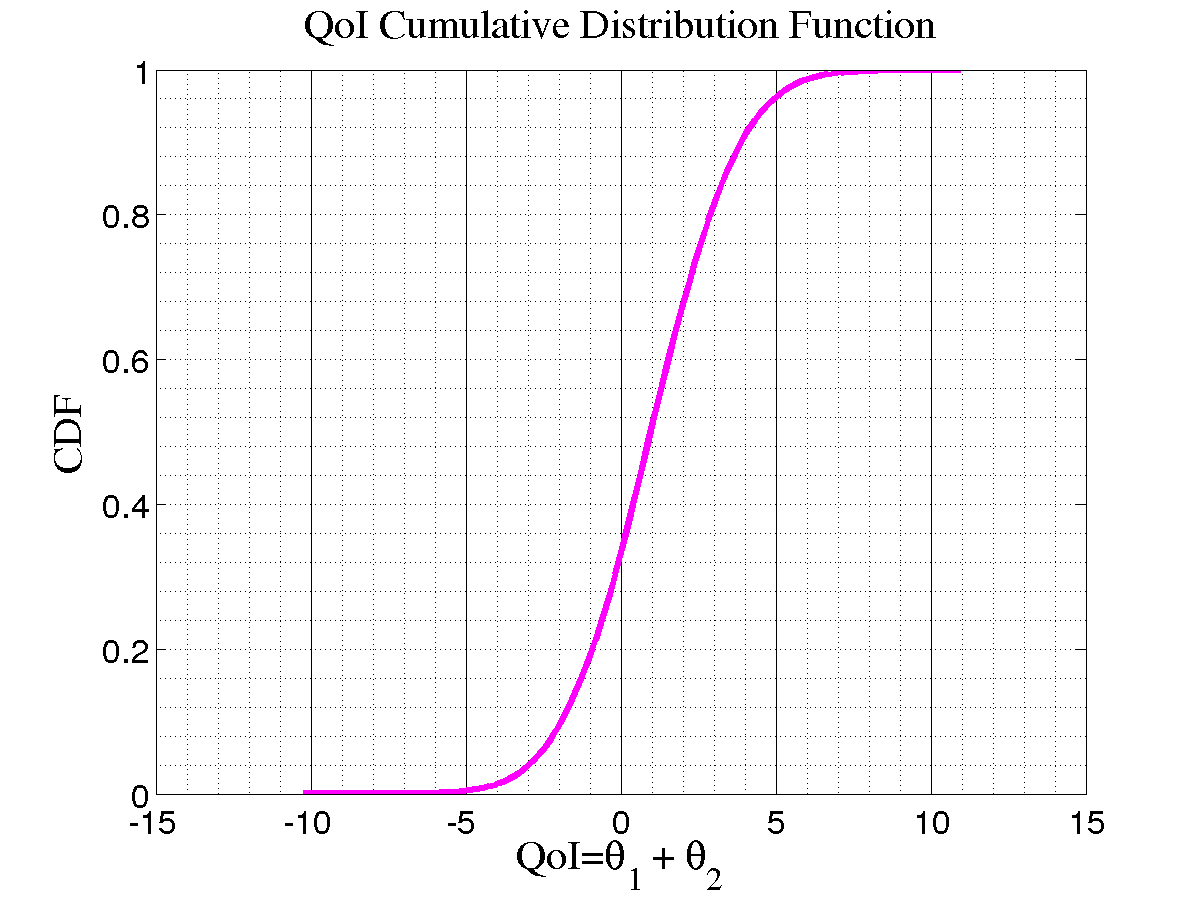
\includegraphics[scale=0.35]{figs/simple_fp_cdf_qoi.png}
\vspace*{-10pt}
\caption{Cumulative Distribution Function.}
\label{fig:simple_sfp_cdf}
\end{figure}
